% Options for packages loaded elsewhere
\PassOptionsToPackage{unicode}{hyperref}
\PassOptionsToPackage{hyphens}{url}
\PassOptionsToPackage{dvipsnames,svgnames,x11names}{xcolor}
%
\documentclass[
  10pt,
  dvipsnames,enabledeprecatedfontcommands]{scrartcl}
\title{Taking uncertainty in word embedding bias estimation seriously: a
bayesian approach}
\author{Alicja Dobrzeniecka and Rafal Urbaniak}
\date{}

\usepackage{amsmath,amssymb}
\usepackage{lmodern}
\usepackage{iftex}
\ifPDFTeX
  \usepackage[T1]{fontenc}
  \usepackage[utf8]{inputenc}
  \usepackage{textcomp} % provide euro and other symbols
\else % if luatex or xetex
  \usepackage{unicode-math}
  \defaultfontfeatures{Scale=MatchLowercase}
  \defaultfontfeatures[\rmfamily]{Ligatures=TeX,Scale=1}
\fi
% Use upquote if available, for straight quotes in verbatim environments
\IfFileExists{upquote.sty}{\usepackage{upquote}}{}
\IfFileExists{microtype.sty}{% use microtype if available
  \usepackage[]{microtype}
  \UseMicrotypeSet[protrusion]{basicmath} % disable protrusion for tt fonts
}{}
\makeatletter
\@ifundefined{KOMAClassName}{% if non-KOMA class
  \IfFileExists{parskip.sty}{%
    \usepackage{parskip}
  }{% else
    \setlength{\parindent}{0pt}
    \setlength{\parskip}{6pt plus 2pt minus 1pt}}
}{% if KOMA class
  \KOMAoptions{parskip=half}}
\makeatother
\usepackage{xcolor}
\IfFileExists{xurl.sty}{\usepackage{xurl}}{} % add URL line breaks if available
\IfFileExists{bookmark.sty}{\usepackage{bookmark}}{\usepackage{hyperref}}
\hypersetup{
  pdftitle={Taking uncertainty in word embedding bias estimation seriously: a bayesian approach},
  pdfauthor={Alicja Dobrzeniecka and Rafal Urbaniak},
  colorlinks=true,
  linkcolor={Maroon},
  filecolor={Maroon},
  citecolor={Blue},
  urlcolor={blue},
  pdfcreator={LaTeX via pandoc}}
\urlstyle{same} % disable monospaced font for URLs
\usepackage{graphicx}
\makeatletter
\def\maxwidth{\ifdim\Gin@nat@width>\linewidth\linewidth\else\Gin@nat@width\fi}
\def\maxheight{\ifdim\Gin@nat@height>\textheight\textheight\else\Gin@nat@height\fi}
\makeatother
% Scale images if necessary, so that they will not overflow the page
% margins by default, and it is still possible to overwrite the defaults
% using explicit options in \includegraphics[width, height, ...]{}
\setkeys{Gin}{width=\maxwidth,height=\maxheight,keepaspectratio}
% Set default figure placement to htbp
\makeatletter
\def\fps@figure{htbp}
\makeatother
\setlength{\emergencystretch}{3em} % prevent overfull lines
\providecommand{\tightlist}{%
  \setlength{\itemsep}{0pt}\setlength{\parskip}{0pt}}
\setcounter{secnumdepth}{5}
\newlength{\cslhangindent}
\setlength{\cslhangindent}{1.5em}
\newlength{\csllabelwidth}
\setlength{\csllabelwidth}{3em}
\newlength{\cslentryspacingunit} % times entry-spacing
\setlength{\cslentryspacingunit}{\parskip}
\newenvironment{CSLReferences}[2] % #1 hanging-ident, #2 entry spacing
 {% don't indent paragraphs
  \setlength{\parindent}{0pt}
  % turn on hanging indent if param 1 is 1
  \ifodd #1
  \let\oldpar\par
  \def\par{\hangindent=\cslhangindent\oldpar}
  \fi
  % set entry spacing
  \setlength{\parskip}{#2\cslentryspacingunit}
 }%
 {}
\usepackage{calc}
\newcommand{\CSLBlock}[1]{#1\hfill\break}
\newcommand{\CSLLeftMargin}[1]{\parbox[t]{\csllabelwidth}{#1}}
\newcommand{\CSLRightInline}[1]{\parbox[t]{\linewidth - \csllabelwidth}{#1}\break}
\newcommand{\CSLIndent}[1]{\hspace{\cslhangindent}#1}
%\documentclass{article}

% %packages
\usepackage{booktabs}
%\usepackage[left]{showlabels}
\usepackage{multirow}
\usepackage{subcaption}

\usepackage{graphicx}
%\usepackage{longtable}
\usepackage{supertabular, booktabs}
\usepackage{ragged2e}
\usepackage{etex}
%\usepackage{yfonts}
\usepackage{marvosym}
\usepackage[notextcomp]{kpfonts}
\usepackage{nicefrac}
\newcommand*{\QED}{\hfill \footnotesize {\sc Q.e.d.}}
\usepackage{floatrow}

\usepackage[textsize=footnotesize]{todonotes}
\newcommand{\ali}[1]{\todo[color=gray!40]{\textbf{Alicja:} #1}}
\newcommand{\mar}[1]{\todo[color=blue!40]{#1}}
\newcommand{\raf}[1]{\todo[color=olive!40]{#1}}

%\linespread{1.5}
\newcommand{\indep}{\!\perp \!\!\! \perp\!}


\setlength{\parindent}{10pt}
\setlength{\parskip}{1pt}


%language
%\usepackage{times}
\usepackage{mathptmx}
\usepackage[scaled=0.86]{helvet}
\usepackage{t1enc}
%\usepackage[utf8x]{inputenc}
%\usepackage[polish]{babel}
%\usepackage{polski}




%AMS
\usepackage{amsfonts}
\usepackage{amssymb}
\usepackage{amsthm}
\usepackage{amsmath}
\usepackage{mathtools}

\usepackage{geometry}
 \geometry{a4paper,left=35mm,top=20mm,}


%environments
\newtheorem{fact}{Fact}



%abbreviations
\newcommand{\ra}{\rangle}
\newcommand{\la}{\langle}
\newcommand{\n}{\neg}
\newcommand{\et}{\wedge}
\newcommand{\jt}{\rightarrow}
\newcommand{\ko}[1]{\forall  #1\,}
\newcommand{\ro}{\leftrightarrow}
\newcommand{\exi}[1]{\exists\, {_{#1}}}
\newcommand{\pr}[1]{\ensuremath{\mathsf{P}(#1)}}
\newcommand{\cost}{\mathsf{cost}}
\newcommand{\benefit}{\mathsf{benefit}}
\newcommand{\ut}{\mathsf{ut}}

\newcommand{\odds}{\mathsf{Odds}}
\newcommand{\ind}{\mathsf{Ind}}
\newcommand{\nf}[2]{\nicefrac{#1\,}{#2}}
\newcommand{\R}[1]{\texttt{#1}}
\newcommand{\prr}[1]{\mbox{$\mathtt{P}_{prior}(#1)$}}
\newcommand{\prp}[1]{\mbox{$\mathtt{P}_{posterior}(#1)$}}



\newtheorem{q}{\color{blue}Question}
\newtheorem{lemma}{Lemma}
\newtheorem{theorem}{Theorem}
\newtheorem{corollary}{Corollary}[fact]


%technical intermezzo
%---------------------

\newcommand{\intermezzoa}{
	\begin{minipage}[c]{13cm}
	\begin{center}\rule{10cm}{0.4pt}



	\tiny{\sc Optional Content Starts}
	
	\vspace{-1mm}
	
	\rule{10cm}{0.4pt}\end{center}
	\end{minipage}\nopagebreak 
	}


\newcommand{\intermezzob}{\nopagebreak 
	\begin{minipage}[c]{13cm}
	\begin{center}\rule{10cm}{0.4pt}

	\tiny{\sc Optional Content Ends}
	
	\vspace{-1mm}
	
	\rule{10cm}{0.4pt}\end{center}
	\end{minipage}
	}
	
	
%--------------------






















\newtheorem*{reply*}{Reply}
\usepackage{enumitem}
\newcommand{\question}[1]{\begin{enumerate}[resume,leftmargin=0cm,labelsep=0cm,align=left]
\item #1
\end{enumerate}}

\usepackage{float}

\usepackage{sectsty}
\sectionfont{\fontsize{11}{11}\selectfont}

% \setbeamertemplate{blocks}[rounded][shadow=true]
% \setbeamertemplate{itemize items}[ball]
% \AtBeginPart{}
% \AtBeginSection{}
% \AtBeginSubsection{}
% \AtBeginSubsubsection{}
% \setlength{\emergencystretch}{0em}
% \setlength{\parskip}{0pt}






\usepackage[authoryear]{natbib}

%\bibliographystyle{apalike}



\usepackage{tikz}
\usetikzlibrary{positioning,shapes,arrows}

\ifLuaTeX
  \usepackage{selnolig}  % disable illegal ligatures
\fi

\begin{document}
\maketitle

\hypertarget{cosine-based-measures-of-bias}{%
\section{Cosine-based measures of
bias}\label{cosine-based-measures-of-bias}}

\hypertarget{word-embeddings-and-their-bias}{%
\subsection{Word embeddings and their
bias}\label{word-embeddings-and-their-bias}}

\begin{itemize}
\tightlist
\item
  akapit filozoficzny, z odniesieniem do value free
\end{itemize}

Modern Natural Language Processing (NLP) models are used to complete
various tasks such as providing email filters, smart assistants, search
results, language translations, text analytics and so on. All of them
need as an input words represented by means of numbers which is
accomplished with word embeddings, in which particular lexical units are
represented as vectors of real numbers.

\begin{itemize}
\item
  troche o tym jak sa skonstruowane (optimizing for co-ocurrence
  frequency)
\item
  przejrzec jak to jest wprowadzane w kilku innych artykulach, zwl. fair
  is better than sensational
\item
  troche wiecej o tej konstrukcji i intuicji semantycznych, ale to nie
  super dobry pomysl
\item
  undesirable bias with respect to a certain groups words if
  stereotypically connected words (for stereotypes that we don't want to
  be used or relied on in downstream tasks) are systematically closer to
  each other. + EXAMPLES
\end{itemize}

It has been suggested {[}1--6{]} that in the learning process such
models can learn implicit biases that reflect harmful stereotypical
thinking. A large chunk of the literature on the topic focuses on the
geometry of the learnt word embeddings; in particular, unusually low
(cosine) proximity of words belonging, intuitively, to a stereotype, is
taken as a sign that this stereotype has been built into a given
embedding. This methodology will be in the focus of our paper.

\hypertarget{general-challenges}{%
\subsection{General challenges}\label{general-challenges}}

\hypertarget{weat-and-mac}{%
\subsection{WEAT and MAC}\label{weat-and-mac}}

One of the first measures in the discussion has been developed by
{[}1{]}. First, the gender direction \(gd\) in is obtained by taking the
differences of the vectors corresponding to ten different gendered pairs
(such as \(\overrightarrow{she} - \overrightarrow{he}\) or
\(\overrightarrow{girl} - \overrightarrow{boy}\)) and then identifying
their principal component (which is the vector obtained by projecting
the data points on their linear combination in a way that maximizes the
variance of the projections).\footnote{In the notebook associated with
  the paper, the authors simply use
  \(\overrightarrow{she} - \overrightarrow{he}\) as a gender direction,
  though.} The gender bias of a word \(w\) is understood as its
projection on the gender direction: \(\vec{w} \cdot gd\). Given the
supposedly gender neutral words \(N\)\footnote{We follow the methodology
  in assuming that there is a class of words that ideally should be
  identified as neutral, such as
  \emph{ballpark, solution, lecture, science, book} can be identified.
  We will have a bit to say about this assumption when we describe our
  dataset construction.} \todo{get back to this!} and the gender
direction \(gd\) the direct gender bias is defined as the average cosine
similarity of the words in \(N\) from \(gd\) (\(c\) is a parameter
determining how strict we want to be):

\footnotesize

\begin{align}
\mathsf{directBias_c(N,gd)} & = \frac{\sum_{w\in N}\vert \mathsf{cos}(\vec{w},gd)\vert^c}{\vert N \vert }
\end{align} \normalsize  The use of projections has been criticized for
instance by {[}4{]}, who point out that while the distance to the gender
direction might be an indicator of bias, it is only one possible
manifestation of it, and reducing the cosine distance to such a
projection might be insufficient. For instance, ``math'' and
``delicate'' might be in equal distance to a pair of opposed explicitly
gendered words, while being closer to quite different stereotypical
attribute words. Further, it is observed in {[}4{]} that most word pairs
preserve similarity under debiasing meant to minimize projection-based
bias.\footnote{In {[}1{]} another method which involves analogies and
  their evaluations by human users on Mechanical Turk is also used. We
  do not discuss this method in this paper, see its criticism in
  {[}7{]}.}

A measure of bias in word embeddings which does not employ gender
directions, the Word Embedding Association Test (WEAT), has been
proposed in {[}2{]}. The idea is that the bias between two sets of
target words, \(X\) and \(Y\) (we call them protected words), should be
quantified in terms of the cosine similarity between the protected words
and attribute words coming from two sets of stereotype attribute words,
\(A\) and \(B\) (we'll call them attributes). For instance, \(X\) might
be a set of male names, \(Y\) a set of female names, \(A\) might contain
stereotypically male-related, and \(B\) stereotypically female-related
career words. The association difference for a term \(t\) is:

\vspace{-2mm}

\footnotesize

\begin{align}
\mathsf{s}(t,A,B) & = \frac{\sum_{a\in A}\mathsf{cos}(t,a)}{\vert A\vert} - \frac{\sum_{b\in B}\mathsf{cos}(t,b)}{\vert B\vert}
\end{align} \normalsize \noindent then, the association difference
between \(A\) a \(B\) is:

\vspace{-2mm}

\footnotesize

\begin{align}
\mathsf{s}(X,Y,A,B) & = \sum_{x\in X} \mathsf{s}(x,A,B) -  \sum_{y\in Y} \mathsf{s}(y,A,B)
\end{align} \normalsize

The effect size is computed by normalizing the difference in means as
follows:\footnote{ WEAT is a modification of the Implicit Association
  Test (IAT) {[}8{]} used in psychology, and it uses almost the same
  word sets, allowing for a \emph{prima facie} sensible comparison with
  bias in humans. {[}2{]} argue that significant biases---thus
  measured--- similar to the ones discovered by IAT can be discovered in
  word embeddings. {[}5{]} extended the methodology to a multilingual
  and cross-lingual setting, arguing that using Euclidean distance
  instead of similarity does not make much difference, while the bias
  effects vary greatly across embedding models (interestingly, with
  social media-text trained embeddings being less biased than those
  based on Wikipedia).}\(^{, }\)\footnote{ A similar methodology is
  employed in {[}3{]}. The authors employ word embeddings trained on
  corpora from different decades to study the shifts in various biases.
  For instance, to compute the occupational embeddings bias for women
  the authors first compute the average vector of vector embeddings of
  words that represent women (e.g.~\emph{she}, and \emph{female}), then
  calculate the Euclidean distance between this mean vector and words
  for occupations. Then they take the mean of these distances and
  subtract from it the analogously obtained mean for the average vector
  of vector embeddings of words that represent men. Formally they take
  the relative norm distance between \(X\) and \(Y\) to be:}

\vspace{-2mm}

\footnotesize

\begin{align}
\mathsf{weat}(A,B) & = \frac{
\mu(\{\mathsf{s}(x,A,B)\}_{x\in X}) -\mu(\{\mathsf{s}(y,A,B)\}_{y\in Y}) 
}{
\sigma(\{\mathsf{s}(w,A,B)\}_{w\in X\cup Y})
}
\end{align}

\normalsize

WEAT, however, has been developed to investigate biases corresponding to
a pair of supposedly opposing stereotypes, and so the question arises as
to how generalize the measure to contexts in which biases with respect
to more than two stereotypical groups are to be measured. Such a
generalization can be found in {[}6{]}. The authors introduce Mean
Average Cosine similarity as a measure of bias (strictly speaking, in
the paper they report cosine distances\footnote{By the cosine distance
  in the literature the authors mean 1-cosine similarity; note however
  that this terminology is slightly misleading, as mathematically it is
  not a distance measure, because it does not satisfy the triangle
  inequality, as generally \(dist(A,C) \not \leq dist(A,B)+ dist(B,C)\);
  we'll keep using this mainstream terminology though.} rather than
similarities). Let \(T = \{t_1, \dots, t_k\}\) be a class of protected
word embeddings, and let each \(A_j\in A\) be a set of attributes
stereotypically associated with a protected word). Then:

\vspace{-2mm }
\footnotesize

\begin{align}
\mathsf{s}(t_i, A_j) & = \frac{1}{\vert A_j\vert}\sum_{a\in A_j}\mathsf{cos}(t,a) \\
\mathsf{mac}(T,A) & = \frac{1}{\vert T \vert \,\vert A\vert}\sum_{t_i \in T }\sum_{A_j \in A} \mathsf{s}(t_i,A_j)
\end{align}

\normalsize

\noindent That is, for each protected word \(T\) and each attribute
class, they first take the mean for this protected word and all
attributes in a given attribute class, and then take the mean of thus
obtained means for all the protected words.

Having introduced the measures, first, we will introduce a selection of
general problems with this approach, and then we will move on to more
specific but important problems related to the statistical significance
of such measurement. We will focus on WEAT and MAC, as we want to put
issues with the use of projections aside. WEAT will be useful in our
criticism of the statistical methods involved, as it is simpler, so the
explanation and visualizations will be more transparent (and
\emph{mutatis mutandis} this criticism will apply to MAC as well), and
MAC will be useful in the development of our alternative method as its
range of applicability is the widest.

\hypertarget{methodological-problems-with-cosine-based-measures-of-bias}{%
\subsection{Methodological problems with cosine-based measures of
bias}\label{methodological-problems-with-cosine-based-measures-of-bias}}

One issue to consider is the selection of attributes for bias
measurement. The word lists used in the literature are often fairly
small (5-50)\todo{Check Manzani}. While the papers do employ statistical
tests to measure the uncertainty involved, we will later on argue that
these method are not proper for the goal at hand and show that a more
appropriate use of statistical methods leads to estimates of uncertainty
that are rather epistemologically pessimistic.
\todo{sensitivity to choice of words}

Let's think about MAC, using the case of religion-related
stereotypes.\todo{crossref to a list of words an explanation} In the
original paper, words from all three religions were compared against all
of the stereotypes. One reason this is problematic is that no
distinction between cases in which the stereotype is associated with a
given religion, as opposed to the situation in which it is associated
with another one, is made. This is problematic, as not all of the
stereotypical words have to be considered as harmful for all of the
religions. One should investigate the religions separately as some of
them may have stronger harmful associations that others.

The interpretation of the results is also a challenge. In {[}6{]} we can
find summaries of average cosine distances per group (such as gender,
race, or religion). For instance, for religion, here is the relevant
fragment of table:\todo{add p-values in the table}

\todo{kable the table}

\noindent (MAC stand for mean average cosine similarity, although in
reality the the table contains mean cosine distances). What may attract
attention is the fact that the value of cosine distance in ``Biased''
category is already quite high (i.e.~close to 1) even before debiasing.
High cosine distance indicates low cosine similarity between values. One
could think that average cosine similarity equal to approximately 0.141
is not significant enough to consider it as bias. However, the authors
still aim to mitigate such ``bias'' to make the distance even larger.
Methodologically the question is, on what basis is this small similarity
still considered as a proof of the presence of bias, and whether these
small changes are meaningful.

The underlying problem here is that in the paper there is no control
group. One should also include control groups to have a way of comparing
the results for a supposedly stereotyped group with the results for sets
of neutral or human-related neutral words. In our approach later on, we
distinguish between stereotypes associated with a given group,
stereotypes associated with different groups, and introduce control
groups: neutral words and stereotype-free human predicates.

\todo{bliskosc znaczeniowa a ko-okurencja}

\todo{comparison should be made to actual frequencies, to separate bias caused by cosine similarty to upstream bias}

\todo{unclear czy to sie przeklada na downstream effect}

\hypertarget{metrics-that-pre-average-are-a-bad-guide}{%
\subsection{Metrics that pre-average are a bad
guide}\label{metrics-that-pre-average-are-a-bad-guide}}

In contrast, statistical intervals will help us decide whether a given
cosine similarity is high enough to consider the words to be more
similar than if we chose them at random. We will use highest posterior
density intervals, in line with Bayesian methodology.

Crucially, these approaches use means of mean average cosine
similarities to measure similarity between protected word and harmful
stereotypes. If one takes a closer look at the individual values that
are taken for the calculations, it turns out that there are quite a few
outliers and surprisingly dissimilar words. This issue will become
transparent when we inspect the visualizations of individual cosine
distances, following the idea that one of the first step to understand
data is to look at it.

With such a method the uncertainty involved is not really considered
which makes it even more difficult to give reasonable interpretations of
the results. We propose the use of Bayesian method to obtain some
understanding of the influence the uncertainty has on the interpretation
of final results.

\todo{odleglosc nie musi uchwytywac relacji semantycznej zeby oceniac bias}

\todo{zalozenie, bardziej ze jezeli odleglosci przekladaja sie na downstream, to warto patrzec na odleglosci, nawet bez glebszej filozoficznej interpretacji ich}

\noindent \(s(X,Y,A,B)\) is the statistic used in the significance test,
and the \(p\)-value is obtained by bootstrapping: it is the frequency of
\(s(X_i,Y_i,A,B)>s(X,Y,A,B)\) for all equally sized partitions
\(X_i, Y_i\) of \(X\cup Y\). The effect size is computed by normalizing
the difference in means as follows:

\vspace{-2mm}

\footnotesize

\begin{align}
bias(A,B) & = \frac{
\mu(\{s(x,A,B)\}_{x\in X}) -\mu(\{s(y,A,B)\}_{y\in Y}) 
}{
\sigma(\{s(w,A,B)\}_{w\in X\cup Y})
}
\end{align}

\normalsize

The t-tests they employ are run on average cosines used to calculate
MAC.

\hypertarget{pre-averaging-and-manufactured-certainty}{%
\section{Pre-averaging and manufactured
certainty}\label{pre-averaging-and-manufactured-certainty}}

\hypertarget{general-problem-with-pre-averaging}{%
\subsection{General problem with
pre-averaging}\label{general-problem-with-pre-averaging}}

\hypertarget{simulations-for-weat}{%
\subsection{Simulations for WEAT}\label{simulations-for-weat}}

\hypertarget{simulations-for-mac}{%
\subsection{Simulations for MAC}\label{simulations-for-mac}}

\hypertarget{bayesian-method}{%
\section{Bayesian method}\label{bayesian-method}}

\hypertarget{bernstein-approach}{%
\subsection{Bernstein approach}\label{bernstein-approach}}

\hypertarget{chasing-metrics}{%
\subsection{Chasing metrics}\label{chasing-metrics}}

\hypertarget{bayesian-method-introduction}{%
\subsection{Bayesian method
introduction}\label{bayesian-method-introduction}}

\hypertarget{existing-applications-to-nlp-and-perhaps-to-bias}{%
\subsection{Existing applications to NLP and perhaps to
bias}\label{existing-applications-to-nlp-and-perhaps-to-bias}}

\hypertarget{model}{%
\subsection{Model}\label{model}}

\hypertarget{results}{%
\section{Results}\label{results}}

\vspace{1mm}
\footnotesize

\begin{figure}


\begin{center}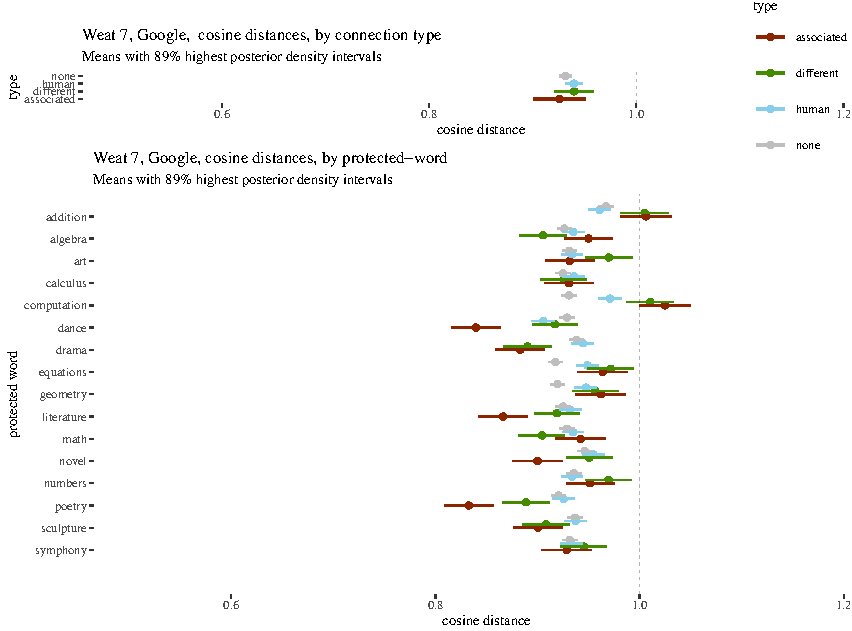
\includegraphics[width=1.1\linewidth]{paperDraft5_files/figure-latex/unnamed-chunk-1-1} \end{center}
\caption{dsds}
\label{fig:weat7google}
\end{figure}

\hypertarget{discussion-and-summary}{%
\section{Discussion and summary}\label{discussion-and-summary}}

\hypertarget{appendix}{%
\section{APPENDIX}\label{appendix}}

\hypertarget{examples-of-weat-and-mac-calculations}{%
\subsection{Examples of WEAT and MAC
calculations}\label{examples-of-weat-and-mac-calculations}}

\hypertarget{word-lists}{%
\subsection*{Word lists}\label{word-lists}}
\addcontentsline{toc}{subsection}{Word lists}

\hypertarget{refs}{}
\begin{CSLReferences}{0}{0}
\leavevmode\vadjust pre{\hypertarget{ref-Bolukbasi2016man}{}}%
\CSLLeftMargin{{[}1{]} }
\CSLRightInline{Tolga Bolukbasi, Kai-Wei Chang, James Y. Zou, Venkatesh
Saligrama, and Adam Kalai. 2016. Man is to computer programmer as woman
is to homemaker? Debiasing word embeddings. \emph{CoRR} abs/1607.06520,
(2016). Retrieved from \url{http://arxiv.org/abs/1607.06520}}

\leavevmode\vadjust pre{\hypertarget{ref-Caliskan2017semanticsBiases}{}}%
\CSLLeftMargin{{[}2{]} }
\CSLRightInline{Aylin Caliskan, Joanna J. Bryson, and Arvind Narayanan.
2017. Semantics derived automatically from language corpora contain
human-like biases. \emph{Science} 356, 6334 (April 2017), 183--186.
DOI:https://doi.org/\href{https://doi.org/10.1126/science.aal4230}{10.1126/science.aal4230}}

\leavevmode\vadjust pre{\hypertarget{ref-Garg2018years}{}}%
\CSLLeftMargin{{[}3{]} }
\CSLRightInline{Nikhil Garg, Londa Schiebinger, Dan Jurafsky, and James
Zou. 2018. Word embeddings quantify 100 years of gender and ethnic
stereotypes. \emph{Proceedings of the National Academy of Sciences} 115,
16 (April 2018), E3635--E3644.
DOI:https://doi.org/\href{https://doi.org/10.1073/pnas.1720347115}{10.1073/pnas.1720347115}}

\leavevmode\vadjust pre{\hypertarget{ref-Gonen2019lipstick}{}}%
\CSLLeftMargin{{[}4{]} }
\CSLRightInline{Hila Gonen and Yoav Goldberg. 2019. Lipstick on a pig:
{D}ebiasing methods cover up systematic gender biases in word embeddings
but do not remove them. In \emph{Proceedings of the 2019 conference of
the north {A}merican chapter of the association for computational
linguistics: Human language technologies, volume 1 (long and short
papers)}, Association for Computational Linguistics, Minneapolis,
Minnesota, 609--614.
DOI:https://doi.org/\href{https://doi.org/10.18653/v1/N19-1061}{10.18653/v1/N19-1061}}

\leavevmode\vadjust pre{\hypertarget{ref-Lauscher2019multidimensional}{}}%
\CSLLeftMargin{{[}5{]} }
\CSLRightInline{Anne Lauscher and Goran Glavas. 2019. Are we
consistently biased? Multidimensional analysis of biases in
distributional word vectors. \emph{CoRR} abs/1904.11783, (2019).
Retrieved from \url{http://arxiv.org/abs/1904.11783}}

\leavevmode\vadjust pre{\hypertarget{ref-Manzini2019blackToCriminal}{}}%
\CSLLeftMargin{{[}6{]} }
\CSLRightInline{Thomas Manzini, Yao Chong Lim, Yulia Tsvetkov, and Alan
W Black. 2019. Black is to criminal as caucasian is to police: Detecting
and removing multiclass bias in word embeddings. Retrieved from
\url{https://arxiv.org/abs/1904.04047}}

\leavevmode\vadjust pre{\hypertarget{ref-Nissim2020fair}{}}%
\CSLLeftMargin{{[}7{]} }
\CSLRightInline{Malvina Nissim, Rik van Noord, and Rob van der Goot.
2020. Fair is better than sensational: Man is to doctor as woman is to
doctor. \emph{Computational Linguistics} 46, 2 (June 2020), 487--497.
DOI:https://doi.org/\href{https://doi.org/10.1162/coli_a_00379}{10.1162/coli\_a\_00379}}

\leavevmode\vadjust pre{\hypertarget{ref-Nosek2002harvesting}{}}%
\CSLLeftMargin{{[}8{]} }
\CSLRightInline{Brian A. Nosek, Mahzarin R. Banaji, and Anthony G.
Greenwald. 2002. Harvesting implicit group attitudes and beliefs from a
demonstration web site. \emph{Group Dynamics: Theory, Research, and
Practice} 6, 1 (2002), 101--115.
DOI:https://doi.org/\href{https://doi.org/10.1037/1089-2699.6.1.101}{10.1037/1089-2699.6.1.101}}

\end{CSLReferences}

\end{document}
